\section{Justering ift. matematisk model af PTS}
Som beskrevet i afsnit \ref{ss:ValgReg} er det valgt at implementere to PI-regulatorer.
Der tages udgangspunkt i den matematiske model af systemet, bestående af overføringsfunktionerne
\(G_{tilt,zoh}\) og \(G_{pan,zoh}\), som er diskretiseringer af de kontinuerte overføringsfunktioner.
Der skal findes to sæt koefficienter, \(K_P\) og \(K_I\), et sæt til hver regulator.
For at medtage den væsentligste ulinearitet, dødzonen, i regulatordesignet,
er det valgt at simulere systemet i Simulink.
I Simulink er den diskretiserede overføringsfunktion indsat sammen med en model for dødzonen,
målt eksperimentelt, samt PI-regulatoren.
Da modellen indeholder ulineariteter er det valgt at starte med et simpelt gain \(K_P\) på 1,
og med Trial-and-Error metoden prøve sig frem til koefficienterne.
Begge regulatorer gives et parabelinput, og deres performance vurderes
efter deres evne til at følge parablen. Dvs. det er forsøgt at minimere Tracking fejlen.

Med ovenstående metode blev koefficienterne i tabel \ref{tb:pidSimulink} fundet tilfredsstillende.
Koefficienterne i tabel \ref{tb:pidSimulink} benævnes startkoefficienterne, da regulatorjusteringen
ift. det fysiske system starter med disse værdier.
Tracking fejlen er afbildet i figur \ref{fig:pidSim1}, og som det ses af grafen, når den maks. 0,5 \degree{} i simuleringen.

\begin{figure}[h!]
\centering
\begin{tabu}{l|[1.25pt]c|c|c}
      & \(K_P\) & \(K_I\) & \(K_D\)\\\tabucline[1.25pt]{-}
Tilt  & 240 & 85 & -\\\hline%0,248960\\\hline
Pan   & 240 &  100 & -
\end{tabu}
\captionsetup{type=table}
\caption[Regulatorkoefficienter]{Koefficienter fundet vha. simulering.}
\label{tb:pidSimulink} 
\end{figure}

\begin{figure}[h!]
\centering
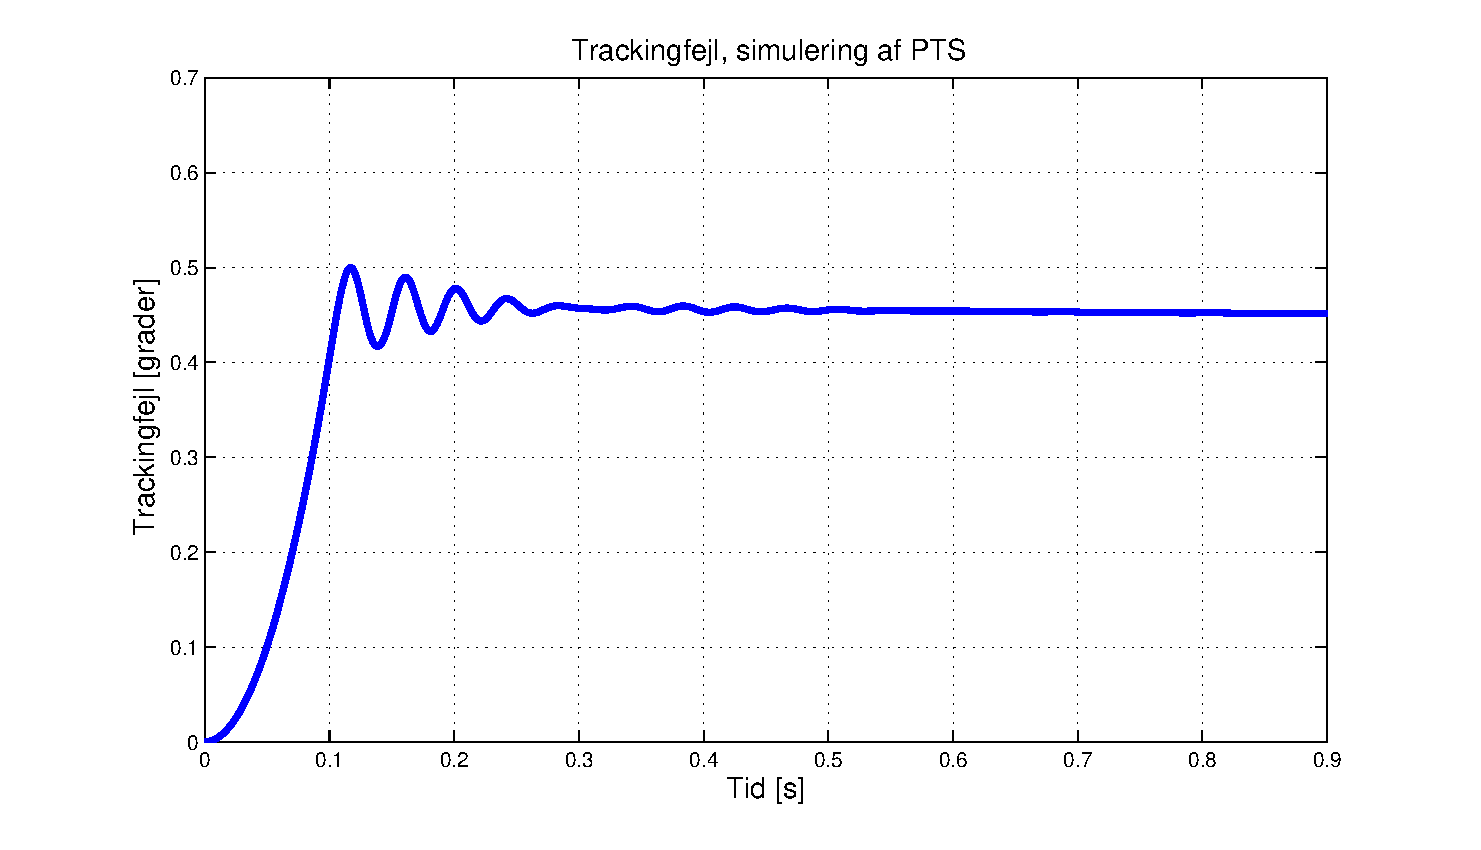
\includegraphics[width=1\textwidth]{./graphics/pidSim1.eps}
\caption[Tracking fejl ved simulering]{Tracking fejl ved simulering af PTS med regulatorkoefficienterne fra tabel \ref{tb:pidSimulink}.} 
\label{fig:pidSim1}
\end{figure}

De to regulatorer er med startkoefficienterne blevet afprøvet i praksis.
Figurer \ref{fig:pidPhys1} viser Pan-fejlsignalet (rød) og Tilt-fejlsignalet (blå)
i forhold til den kontinuerte lerdueparabel fra applikationen.

\begin{figure}[h!]
\centering
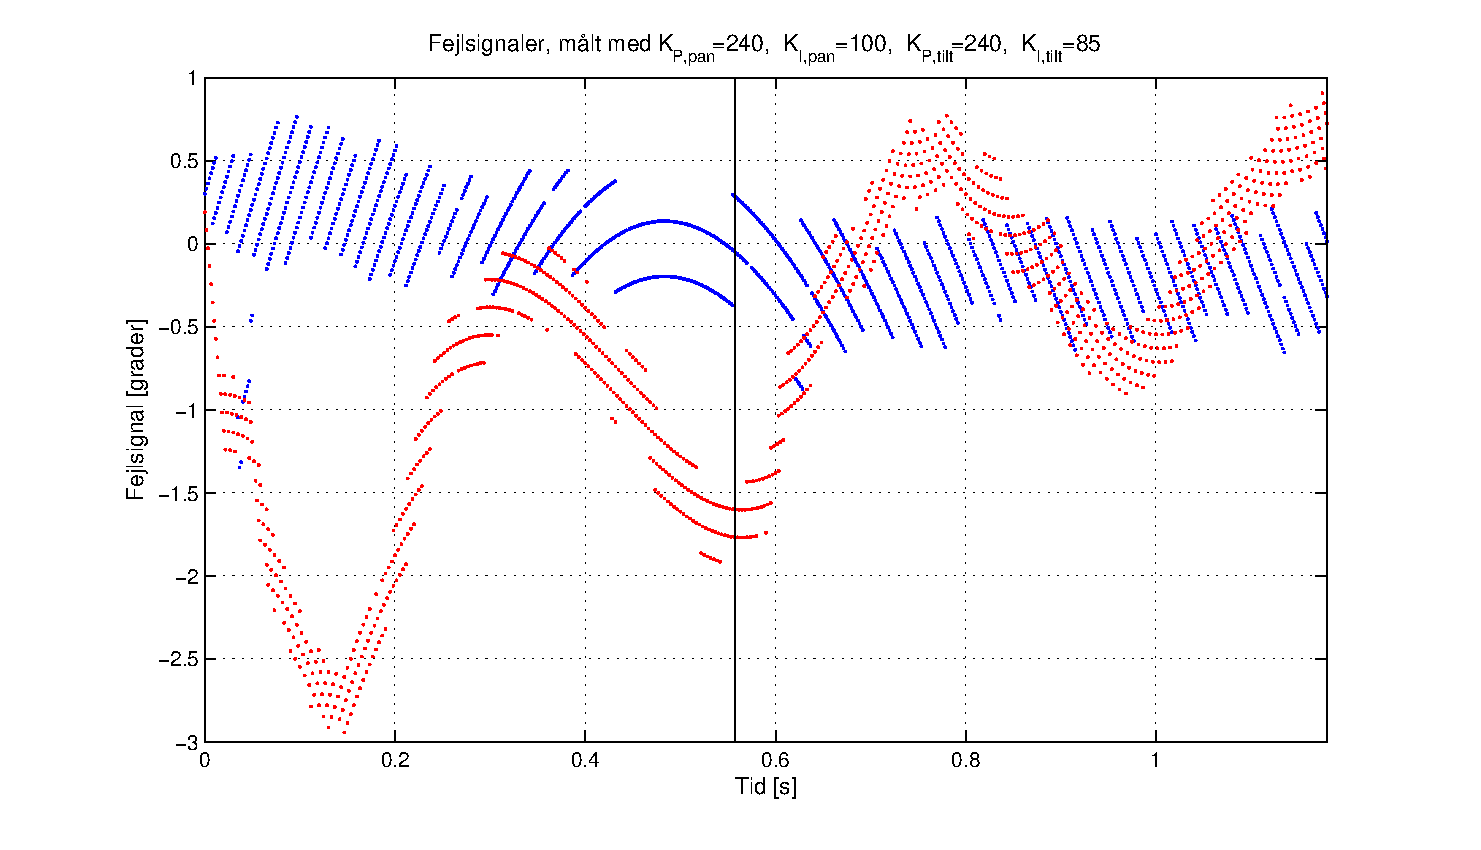
\includegraphics[width=1\textwidth]{./graphics/pidPhys1.eps}
\caption[Fejlsignaler m. startkoefficienter]{Fejlsignaler m. startkoefficienterne fra tabel \ref{tb:pidSimulink}.
	De sorte lodrette streger angiver \(t_s=0,557 \text{ [s]}\).\\
	Pan-fejlsignalet er markeret med prikker, og Tilt-fejlsignalet er markeret med krydser.} 
\label{fig:pidPhys1}
\end{figure}

Som det ses på figur \ref{fig:pidPhys1} giver regulatoren til Tilt et fejlsignal,
der maks. afviger 0,9 \degree{} fra 0.
Pan-fejlen afviger derimod op til 1,8 \degree{} pga. et for højt overshoot.
Tracking fejlen er altså langt større end kravet på maksimalt 1,02 \degree.
En manuel justering af koefficienterne på især Pan-regulatoren er derfor nødvendig.

\section{Manuel justering ift. fysisk PTS}

Ved at ændre på koefficienterne og analysere fejlgraferne justeres performance 
hen mod det ønskede.

Det ses at trackingfejlkravet kan opfyldes med en PI regulator på tilt.
På pan er der behov for en hurtigere reaktion, hvilket medfører et større overshoot. 
For at mindske overshootet vurderes det, at der på pan er behov for en PID 
regulator.

\todo[inline,color=Pink,author=Mikkel]{Ovenstående er meget kvalitativt -  men alternativet er at vi skal have en del grafer, som let kommer til at fylde mange sider.}

\subsection{Valg af integratormætning}
Det vælges at sætte integratormætningen til 100 for begge regulatorer betyder, da det vurderes, at der drages
fuld nytte af integratorleddet, da ligning \ref{eq:integratorsaturation} 
overholdes.

\begin{equation}
	K_I \cdot Integrator_{Max} > PWM_{Max}
\label{eq:integratorsaturation} 
\end{equation}

\todo[inline,color=Pink,author=Mikkel]{Måske for kvalitativt. Måske må man ikke bare lave sin egen ligning, men jeg har ikke nogne kilde.}


\subsection{Tilføjelse af et D-filter}
Det vurderes at kravene for Pan rammen ikke kunne opnåes vha. en standard PID regulator. 
Det vælges derfor at tilføje et filter til D-leddet. 
Det betyder at D-leddet nu vægter tidligere ændringer i error signalet. 
Filtret reducerer peaks i det differrencierede errorsignal, der skyldes ZoH i upsamplingen (se afsnit \ref{subsec:upsampling}).

Der implementeres et 4. ordens FIR filter. Filtret er designet i fdatool med brug af at Kaiser vindue. Filtrets step og frekvensrespons kan ses på figur \ref{fig:d_filter_step} hhv. \ref{fig:d_filter_bode}. 

\begin{figure}[h!]
\centering
\subfloat[Steprespons for det implementerede filter.\label{fig:d_filter_step}]{%
	\hspace*{-0.6cm}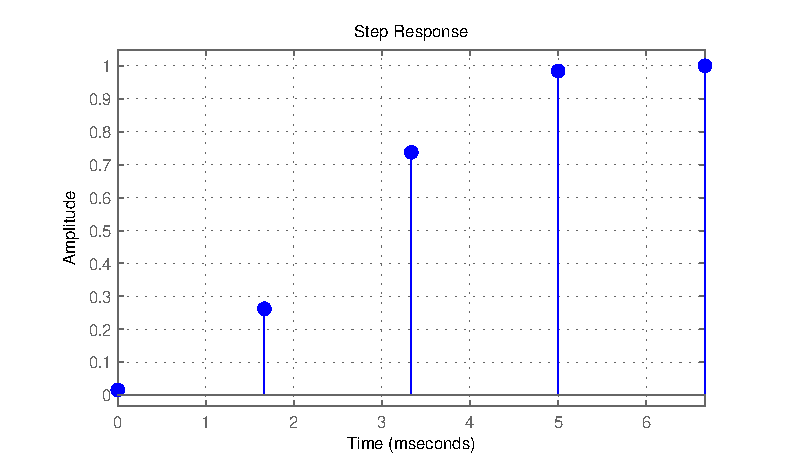
\includegraphics[width=0.57\textwidth]{./graphics/d-filter-step-small}
}
\subfloat[Frekvensrespons for det implementerede filter.\label{fig:d_filter_bode}]{%
	\hspace*{-1.15cm}\includegraphics[width=0.57\textwidth]{./graphics/d-filter-bode-small}
	
}
\caption[D-filterets respons]{Dette er ikke en figur tekst. }
\label{fig:d_filter}
\end{figure}


%[.5\linewidth]{\includegraphics{{./graphics/d-filter-bode-small}}}


%Som det fremgår af figur \ref{fig:PID_test14_plot}, er den samlet tracking fejl XXXXXXXXXXXXXX i 
%forhold til kravene for PTS. Grundet tracking fejlen skal optimeringen af controller koefficienterne
 %foretages manuelt.
%Finjusteringen af controller koefficienterne udføres som en iterativ proces. Optimeringsprocessen 
%er opdelt i to, således der kun foretages ændringer for enten pan eller tilt. 
%Optimerings iterationerne tager udgangspunkt i en grafisk afbildning af tracking fejlen, 
%hvor efter det vurderes hvorledes hver controller koefficient skal øges eller mindskes for at få det ønsket resultat. 
%Der blev foretaget XXXXXXXXXX ilterationer og det lykkes at få en samlet tracking fejl 
%som opfylder kravet, angivet i ligning \ref{eq:ks:trackingerror}.



\section{Endelig performance}
%For ilteration XXXXXXXXX med controller koefficienterne angivet i tabel \ref{tb:PID_final}, er det 
%lykkedes at opfylde kravet om den samlede tracking fejl som stilles for PTS. 
%Figur \ref{fig:PID_final} viser tracking fejlen for hhv. pan og tilt samt den samlede tracking fejl. 

Efter adskillige test og finjustering af regulatoren, vurderes det at 
koefficienterne i tabel \ref{tb:PID_final} giver den bedst mulige performance 
for PTS. Denne performance ses i \ref{fig:PID_final}. Det ses at trackingfejlen 
holder sig inden for de 1,02$\degree$  pånær ved et par enkelte samples.

\begin{figure}[h!]
\centering
\begin{tabu}{l|[1.25pt]c|c|c}
      & \(K_P\) & \(K_I\) & \(K_D\)\\\tabucline[1.25pt]{-}
Tilt  & 49 & 32,5 & 0\\\hline
Pan   & 80 & 160 & 3,55
\end{tabu}
\captionsetup{type=table}
\caption[Endelige regulatorkoefficienter]{De endelige regulatorkoefficienter.}
\label{tb:PID_final} 
\end{figure}

\begin{figure}[h!]
\centering
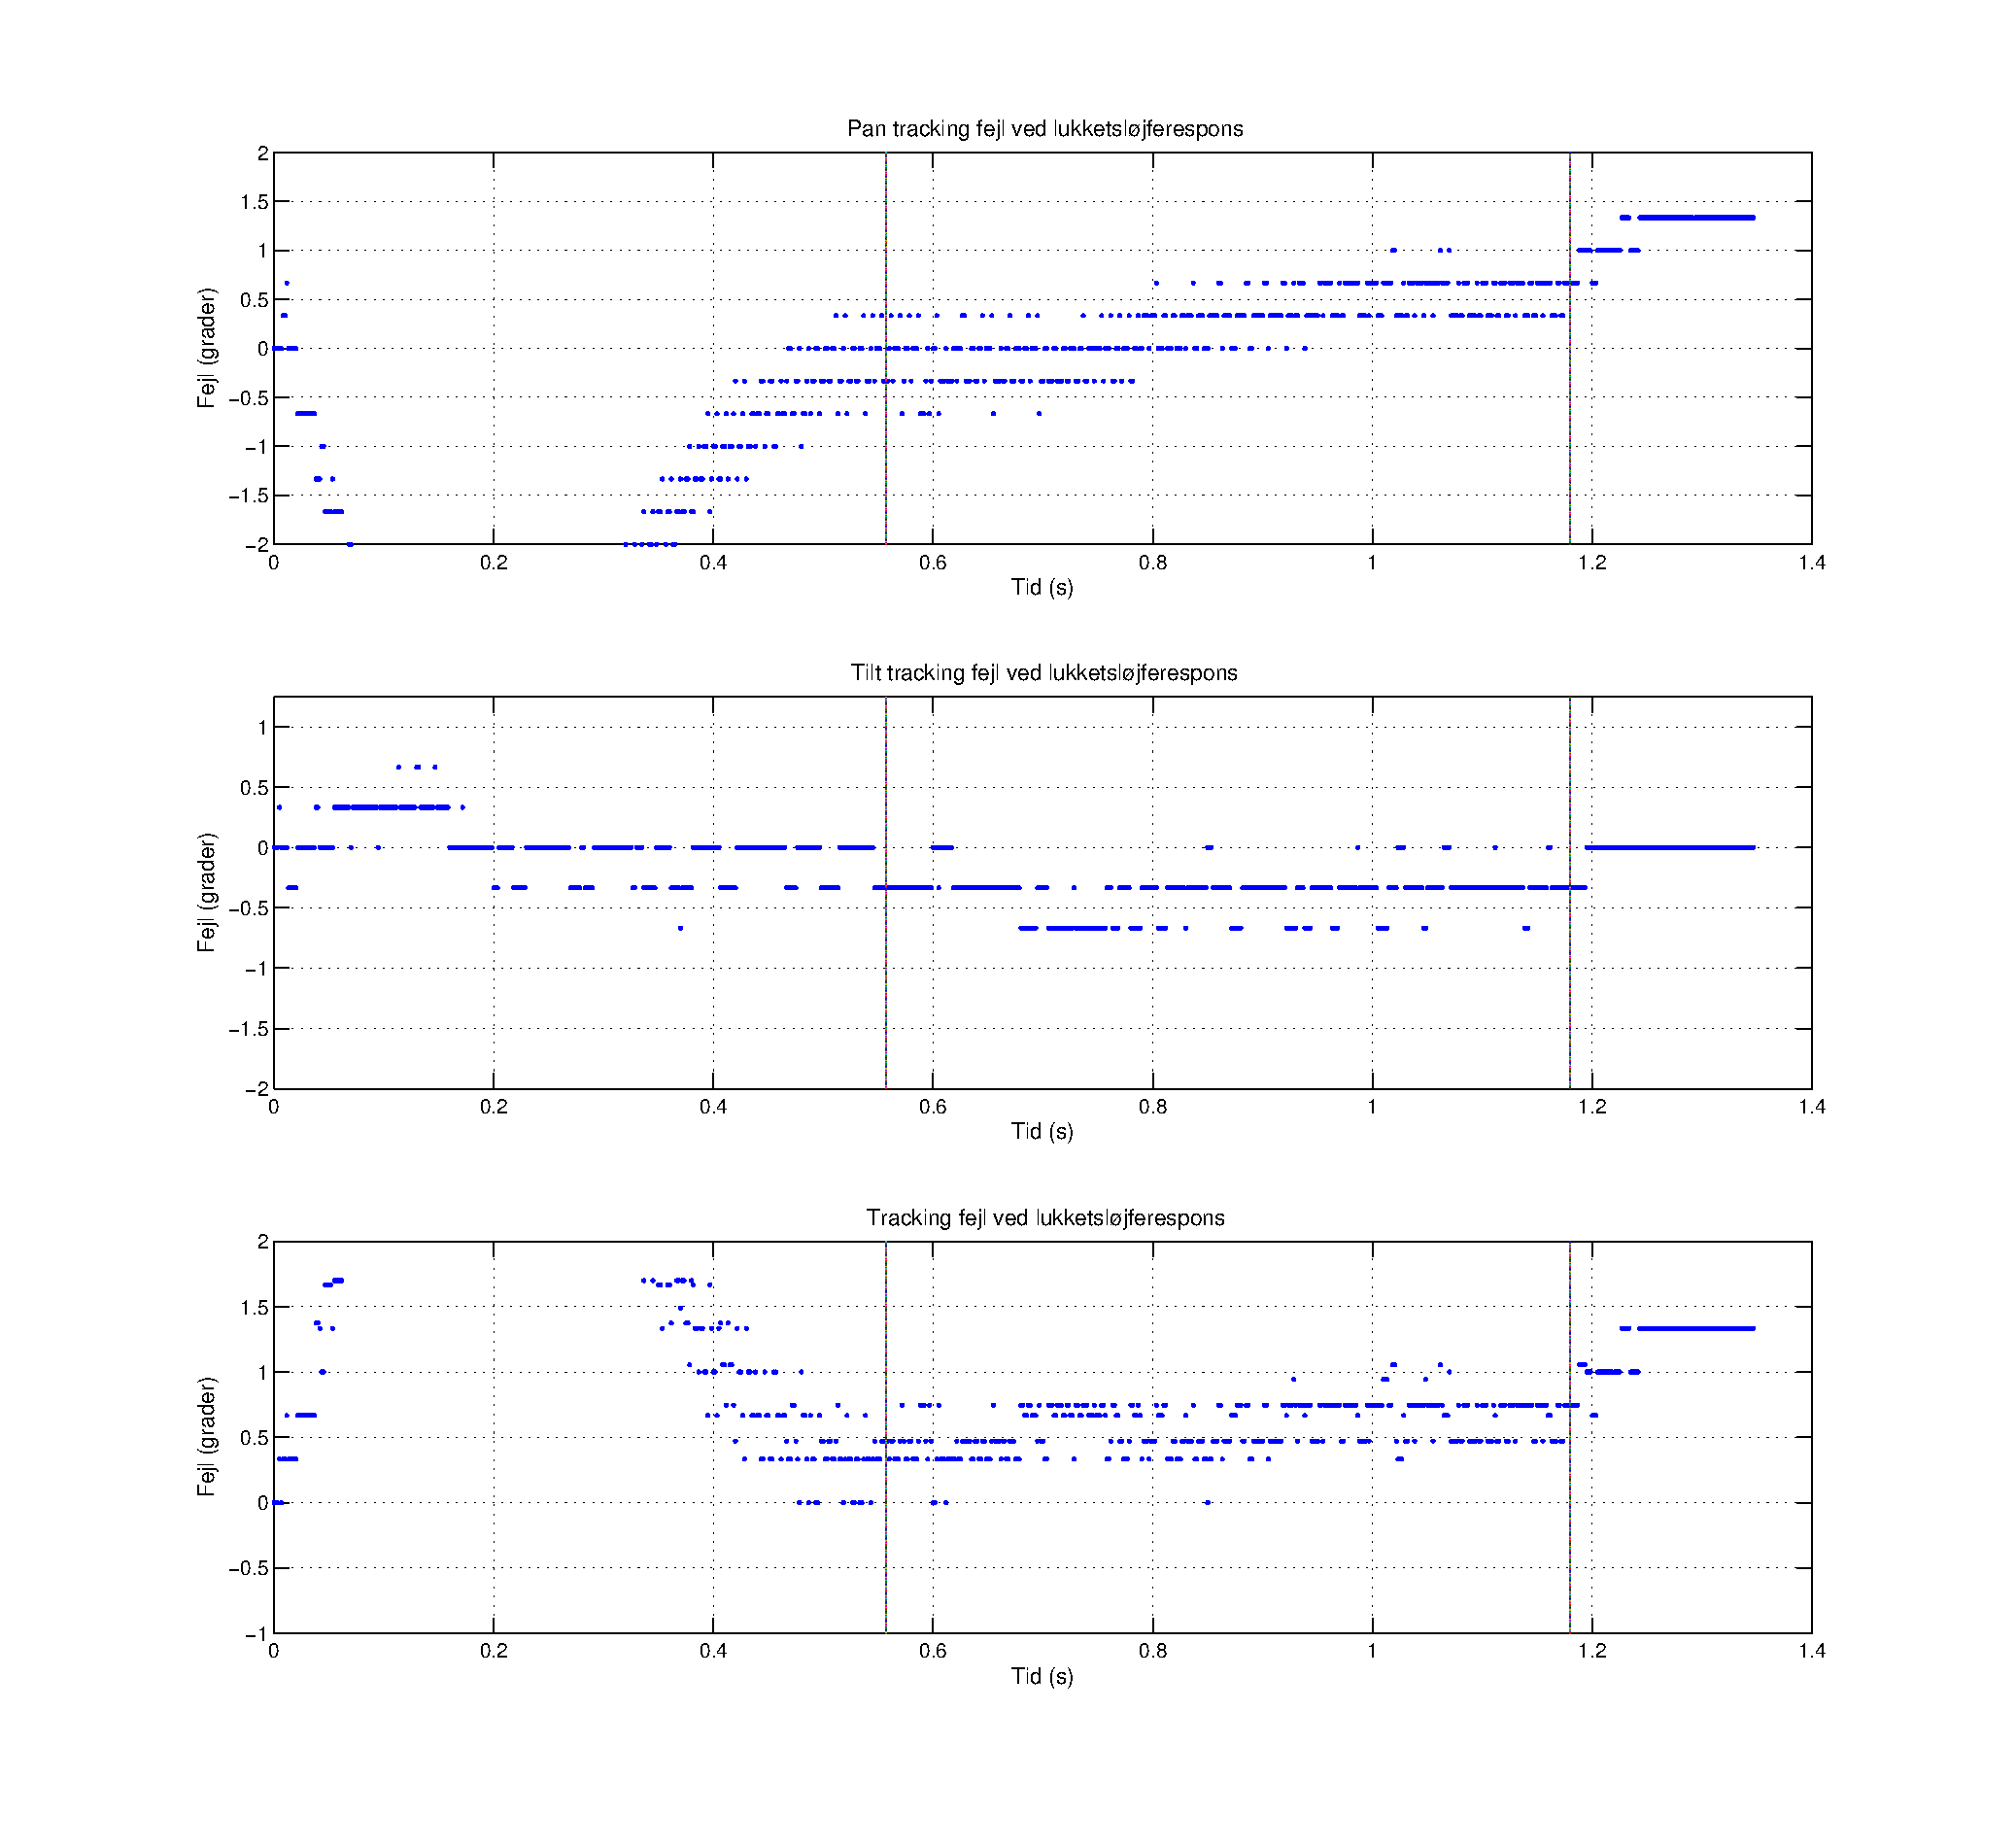
\includegraphics[width=1\textwidth]{./graphics/error_slut.eps}
\caption[Endelig regulator koefficienter]{Tracking fejl målt i grader for hhv. pan og tilt samt den samlet tracking fejl. Testen tager udgangspunkt i koefficienterne fra  tabel \ref{tb:PID_final} og det ses at den samlet tracking fejl opfylder kravet til PTS.} 
\label{fig:PID_final}
\end{figure}

\section{Delkonlusion}
Ved trial \& error blev regulatorkoefficienterne justeret til at give den ønskede 
steprespons. Disse koefficienter giver dårlige performance ved PTS. 
Efter yderligere manuel justering med PI regulator og integratormætning på pan og tilt lykkedes 
det ikke at få den ønskede performance på pan. 
Derfor laves en PID regulator med D-filter til pan. Med denne PID regulator til pan og 
PI regulatoren til tilt opnås den ønskede performance. 
Trackingfejlen holdes under kravet på 1.02 \degree{} pånær ved et par enkelte 
samples.
